\chapter{Conclusioni}
%\markboth{Introduzione}{Introduzione}
\label{cap:conclusioni}


\begin{figure}
\centering
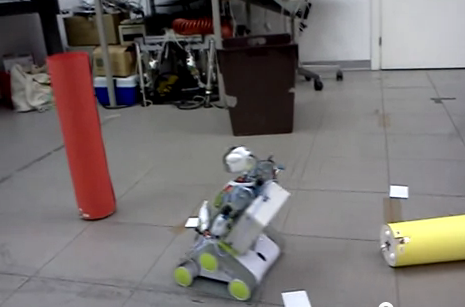
\includegraphics[scale=0.7]{images/attaccotorre}
\caption{Spykee va all'attacco della torre, dopo aver distrutto una fabbrica}
\end{figure}

Dalle prove che abbiamo effettuato, RoboTower risulta giocabile e coinvolgente per il giocatore. Inoltre, variando il numero e la dimensione degli ostacoli fissi, oppure agendo sui parametri di configurazione (tempo del round, tempo di ricarica delle carte, ...) è possibile utilizzare efficacemente il gioco sia in aree di dimensione limitata, che in aree di una dimensione maggiore. Inoltre, variando la dimensione del campo di gioco, viene posto maggiormente l'accento sull'aspetto strategico del gioco (posizionamento corretto degli ostacoli, delle torri e delle fabbriche all'inizio del gioco), oppure su quello dinamico, agendo sul posizionamento delle trappole durante l'avanzata del robot.

Le maggiori problematiche relative all'implementazione del gioco riguardano alcuni limiti degli strumenti a disposizione, in particolare del sistema di visione e del controllo del movimento. Per quanto riguarda la visione, il funzionamento degli algoritmi è fortemente inficiato dalla qualità dell'immagine proveniente dalla telecamera. Le immagini, infatti, a causa della forte compressione JPEG cui sono sottoposte, hanno visibili artefatti che influenzano negativamente il riconoscimento dei blob colorati. Purtroppo, essendo la compressione effettuata a bordo del robot, non è possibile ridurre la compressione. Altri problemi della visione sono legati alla forte dipendenza alle condizioni di luminosità dell'algoritmo di visione utilizzato, che rende necessario effettuare più volte il training del classificatore, a seconda delle condizioni di luce.

Per quanto riguarda il controllo del movimento, l'imprecisione dei comandi ricevuti dal robot rende impossibile, sull'attuale hardware, controllane precisamente l'effetto. Questo provoca dipendenza della risposta del robot ai comandi da molteplici fattori, come la carica della batteria, la superficie su cui si muove, e la frequenza di arrivo dei comandi. Inoltre, a causa di questo problema e della mancanza di opportuni sensori, risulta impossibile creare una mappa dell'ambiente, o più semplicemente mantenere informazioni riguardo le posizioni di alcuni elementi rispetto al robot: questo non permette di attuare strategie complesse, che tengano conto della posizione degli oggetti già visti, e di pianificare in maniera adeguata l'aggiramento degli ostacoli. %mah, secondo me il fatto che è in anello aperto non è assolutamente un problema. Il problema è che (1) ogni invio di comando produce un effetto diverso a seconda di... boh, (2) manca l'odometria. Ho evitato il riferimento all'anello aperto\chiuso: controllo ad anello aperto con odometria permette di attuare strategie complesse finché vuoi; un po' di precisione in piu' nei comandi puoi ottenerla anche con anello aperto, oppure le strategie ad anello chiuso possono essere implementate direttamente dal fw del robot, che riceve controlli ad alto livello esternamente ad anello aperto (non so se mi sono spiegato...)

I maggiori successi nell'implementazione del robot provengono dallo sfruttamento della logica fuzzy e da MrBrian, che ben si adattano a situazioni poco definite, come lo sono i dati che vengono estratti dai sensori del robot. Tramite regole fuzzy, si è riusciti a implementare un comportamento che risponde abbastanza bene agli stimoli dell'ambiente, rendendo il robot in grado di evitare ostacoli in maniera abbastanza soddisfacente e di puntare gli obiettivi seguendo delle traiettorie abbastanza pulite e razionali, nonostante il controllo impreciso dei motori. % ok, eviterei il commento sulle traiettorie abbastanza pulite e razionali... questa parte comunque non so se metterla, starei piu' ad alto livello qui... poi vedi tu

%In particolare i movimenti del robot sono resi più efficaci dalla separazione a livelli delle regole da applicare, feature che permette di disaccoppiare i movimenti come la ricerca e il puntamento degli obiettivi (torri, fabbriche) dalle reazioni ad eventuali stimoli esterni quali ad esempio gli ostacoli fisici. %mah, lo toglierei. la divisione in livelli semplifica l'implementazione, piu' che il comportamento stesso (potresti ottenere lo stesso effetto con regole piu' complesse perché devono tener conto di tutto)

%Altri ottimi risultati sono arrivati grazie alla libreria ROS (Robot Operating System), che nonostante dia molte difficoltà nella configurazione, offre un ottimo middleware sia per l'architettura client/server che per l'architettura publish/subscribe, e fornisce inoltre moltissimi tool grafici e da linea di comando per semplificare il debug e il design delle applicazioni. 
%Inoltre ROS favorisce il disaccoppiamento delle parti del sistema, in quanto ogni "nodo" del sistema è eseguito in un processo separato. Questa feature permette di delocalizzare su macchine differenti l'esecuzione dei nodi, inoltre favorisce la riusabilità dei componenti in quanto risultano debolmente accoppiati. E' facile quindi re-implementare parte del codice per portare RoboTower su altri robot. %ros l'abbiamo gia' spiegato, qui _se parliamo anche degli strumenti utilizzati_ accennerei soltanto [vedi sotto]

Altri ottimi risultati sono arrivati grazie al middleware ROS, che ha consentito un forte disaccoppiamento delle parti del sistema, favorendo la riusabilità dei componenti. È facile quindi re-implementare parte del codice per portare RoboTower su altri robot. Inoltre, fornisce  moltissimi tool grafici e da linea di comando per semplificare il debug e il design delle applicazioni. 

%TODO accennare al riconoscimento giocatore x evitare che si metta davanti alla torre???
